\documentclass{article}
\usepackage[utf8]{inputenc}  
\usepackage[T1]{fontenc}     
\usepackage{graphicx}
\usepackage{amsmath}
\usepackage{pgfplots}
\usepackage{tikz}

\title{Zadanie domowe 4}
\author{Nel Skowronek}
\date{\today}

\begin{document}

\maketitle

\section*{Zadanie 1: Nierówności ogonowe dla rozkładu dwumianowego \text{Bin}\left(n, \frac{1}{2}\right)}

Przybliżymy wartości następujących prawdopodobieństw za pomocą nierówności Markowa i Czebyszewa:
\begin{itemize}
    \item \( P\left(X \geq \frac{6}{5} \cdot \mathbb{E}(X)\right) \)
    \item \( P\left(\left|X - \mathbb{E}(X)\right| \geq \frac{1}{10} \cdot \mathbb{E}(X) \right) \)
\end{itemize}
Aby móc zastosować obie nierówności do obu prawdopodobieństw, trzeba skożystać z faktu, że rozkład \text{Bin}\left(n, \frac{1}{2}\right) jest symetryczny:
\begin{itemize}
    \item \( P\left(X \geq \frac{6}{5} \cdot \mathbb{E}(X)\right) = P\left(X - \mathbb{E}(X) \geq \frac{1}{5} \cdot \mathbb{E}(X)\right) = \frac{1}{2}P\left(\left|X - \mathbb{E}(X)\right| \geq \frac{1}{5} \cdot \mathbb{E}(X)\right) \)
    \item \( P\left(\left|X - \mathbb{E}(X) \right| \geq \frac{1}{10} \cdot \mathbb{E}(X) \right) = 2P\left(X - \mathbb{E}(X) \geq \frac{1}{10} \cdot \mathbb{E}(X) \right) = 2P\left(X \geq \frac{11}{10} \cdot \mathbb{E}(X) \right) \)
\end{itemize}

Wyniki przybliżeń oraz dokładne wartości prawdopodobieństw:
\hspace*{-0cm} 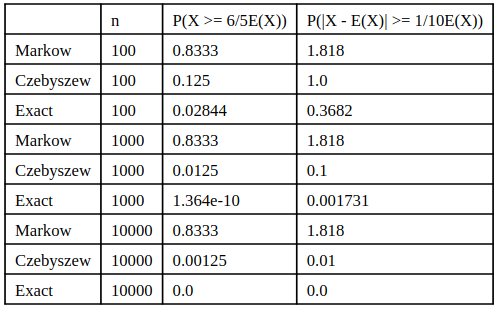
\includegraphics[scale=0.5]{./plots/exc1.png}

Jak widać, obie nierówności zostawiają wiele do życzenia, jednak nierówność Czebyszewa jest zdecydowanie dokładniejsza.
Daje bliższe wyniki, oraz zależy od \text{n}, co nie ma miejsca w nierówności Markowa w tych przypadkach.\\

\section*{Zadanie 2: Błądzenie losowe na liczbach całkowitych}

W celu ułatwienia zadania należy zauważyć, że zmienna \( S_N \) jest transformacją liniową rozkładu \( Bin\left(N, \frac{1}{2}\right) \).
Dokładniej: \\
\( S_N = 2 * Bin\left(n, \frac{1}{2}\right) - N \)\\
A więc: \\
\( F_{S_N}\left(t\right) = P\left(S_N \leq t\right) = P\left(2 * Bin\left(n, \frac{1}{2}\right) - N \leq t\right) = P\left(Bin\left(n, \frac{1}{2}\right) \leq \frac{t + N}{2}\right) \)\\
Wystarczy więc wyznaczyć dystrybuantę \( Bin\left(N, \frac{1}{2}\right) \) i odpowiednio przeskalować pod nią oś \text{OX}.

Wykresy dystrybuant \( S_N \) oraz przybliżających ich rozkładów normalnych \( \mathcal{N}\left(E\left(S_N\right), \sqrt{var\left(S_N\right)}\right) \):
\hspace*{-0cm} 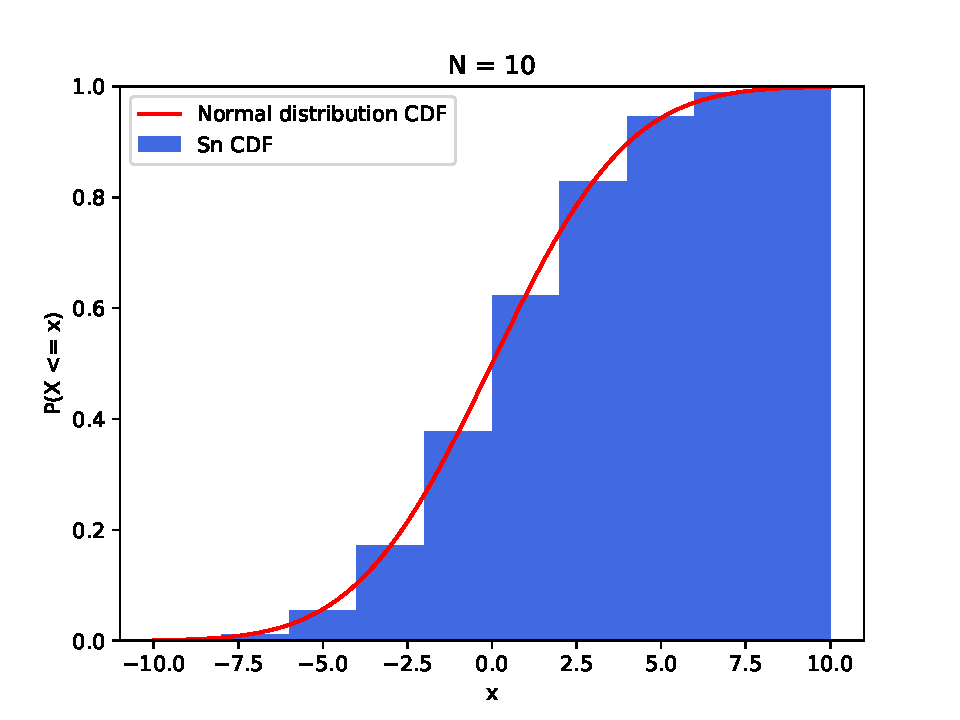
\includegraphics[scale=0.5]{./plots/exc2.pdf}

Wyraźnie widać że razem z rosnącym \( N \), \( S_N \) zbiega według rozkładu do \( \mathcal{N}\left(E\left(S_N\right), var\left(S_N\right)\right) \)\\
co jest zgodne z \textbf{CLT}. \\

\section*{Zadanie 3: Błądzenie losowe na \mathbb{Z} - rozkład \textit{„czasu spędzonego nad osią OX”}}

Wyniki przeprowadzonych symulacji:
\hspace*{-0cm} 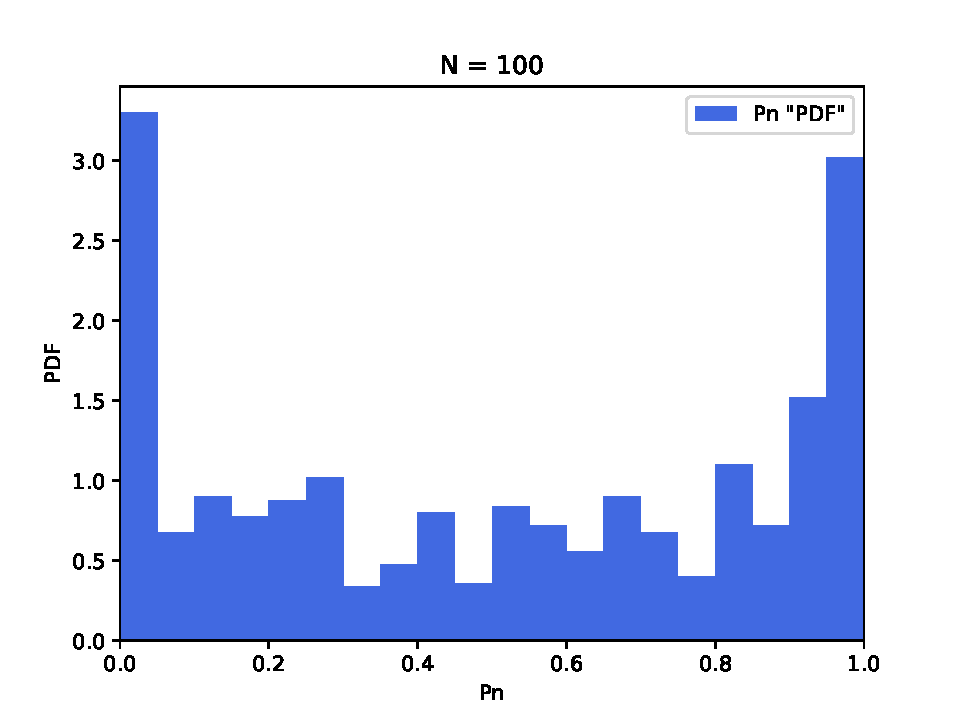
\includegraphics[scale=0.5]{./plots/exc3.pdf}

Dla porównania - funkcja gęstości rozkładu z zadania 5 listy 8 \( \mathcal{f}_X\left(x\right) = \frac{1}{\pi\sqrt{x - x^2}} \):
\hspace*{-0cm} 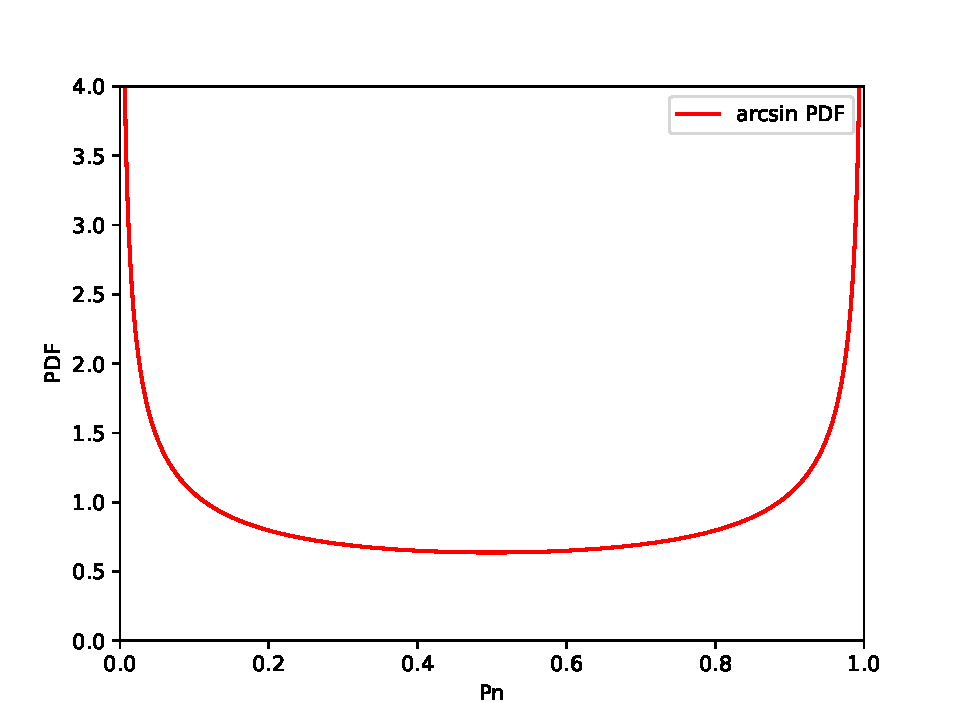
\includegraphics[scale=0.5]{./plots/exc3-arcsin.pdf}

Widać mocne podobieństwo pomiędzy wykresami, co sugerowałoby dążenie rozkładu \( P_N \) do rozkładu arcusa sinusa z zadania 5.
Jedną z rzeczy, które najmocniej rzucają się w oczy jest jednak tendencja do przyjmowania przez \( P_N \) granicznych wartości (0 lub 1).
Interpretacja tego jest taka, że prawie cały spacer spędziliśmy albo nad osią \text{OX} albo pod.
Jest to zgodne z intuicją, z powodu \textit{braku pamięci} procesu \( S_N \) - po oddaleniu się o kilka kroków od osi \text{OX} 
proces \textit{nie pamięta} jakie było jego położenie początkowe. Zachowuje się jakby zaczynał zupełnie od nowa na tej wysokości.
Nic go nie ciągnie spowrotem do osi \text{OX}.

\end{document}
